\documentclass[12pt,letterpaper]{article}

\title{\LARGE Installing Tensorflow on Linux}
%\author{Feiyang Cai}
\date{\today}

\usepackage{listings, lstautogobble}
\usepackage{graphics}
\usepackage[dripdfm]{graphicx}
\usepackage{xcolor}
\usepackage{hyperref}
\hypersetup{
	colorlinks=true,
	linkcolor=red,
	filecolor=magenta,      
	urlcolor=blue,
	urlbordercolor={1 0 0},
	linkbordercolor={1 0 0},
	pdftitle={Sharelatex Example},
	bookmarks=true,
	pdfpagemode=FullScreen,
}

\lstset{ 
	frame = single, 
	language=bash, 
	autogobble=true,
	basicstyle=\small,
	framexleftmargin=0pt}

\usepackage{textcomp}

\usepackage{pythonhighlight}

\begin{document}
	\maketitle
	
	This tutorial introduces how to install TensorFlow on Linux. Here, we installed it on \href{https://www.ubuntu.com/download/desktop}{Ubuntu 16.04} for an example. Also, you can refer to the \href{https://www.tensorflow.org/install/install_linux}{TensorFlow official installation tutorial}. \par
	After installing, we take \hyperref[sec:LinearReg]{linear regression} to explain how to run a TensorFlow program by Python.
	
	\section{Installation}
	\subsection{Determine which TensorFlow to install} \par
	
	There are two types of TensorFlow you can install: CPU support version and GPU support version.\par
	If your system has a NVIDIA\textsuperscript{\textregistered} GPU, you can install the GPU support version. TensorFlow programs typically run significantly faster on a GPU than on a CPU. However, the installation progress of GPU version is more complicated than CPU version, cause you need to install CUDA and cuDNN firstly. \par
	
	On the other hand, if your system doesn't have a NVIDIA\textsuperscript{\textregistered} GPU or you want to simplify the installation progress even if  has a NVIDIA\textsuperscript{\textregistered} GPU, you can install CPU support version.
	
	\subsection{Installing CUDA and cuDNN}
	If you want to install the GPU version TensorFlow, you need to install the CUDA and cuDNN firstly. If you just want to install CPU version, please skip this section to \hyperref[sec:InstallationTensorFlow]{Installing TensorFlow}. \par
	
	\subsubsection{Installing CUDA}
	At first, let we install the CUDA first. Go to the \href{https://developer.nvidia.com/cuda-downloads}{CUDA download page}, and download the CUDA file you need, as the Fig.\ref{Fig:CUDAPage} shown. Here, we download the CUDA\textsuperscript{\textregistered} Toolkit 8.0 for Ubuntu 16.04.
	
	\begin{figure}[http]
		\centering
		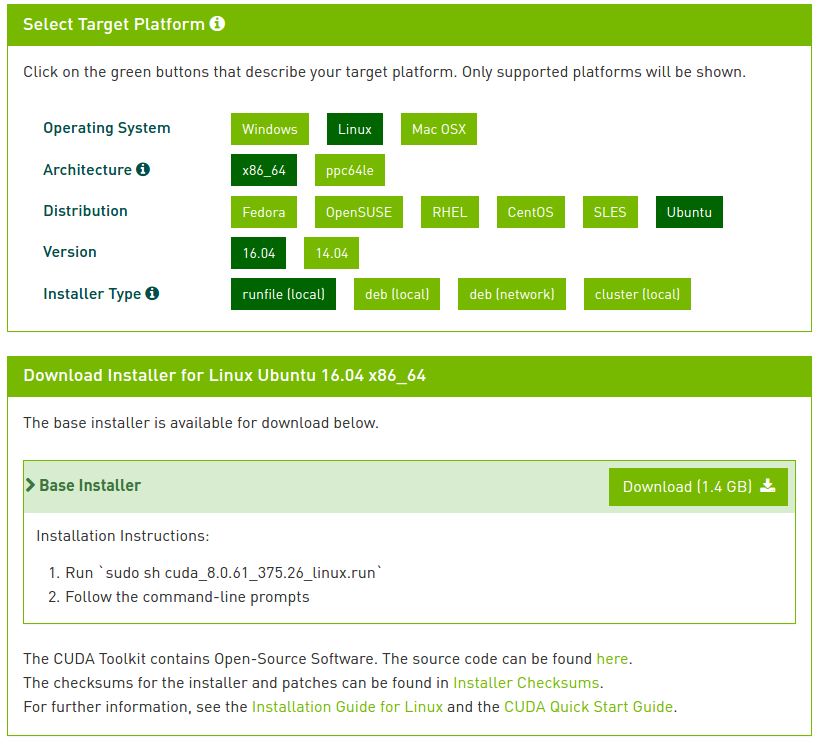
\includegraphics[scale=0.45]{./CUDAPage.png}
		\caption{\label{Fig:CUDAPage}CUDA download page}
	\end{figure}  

	When we finish it, now let's install it. Change to the directories you saved the CUDA file using terminal, and start the installation. The command is shown as below and you can see the terminal as  
	Fig.\ref{Fig:StartCUDA}.
	\begin{lstlisting}{frame=single, language=bash}
	$ cd Desktop/
	$ sudo sh cuda_8.0.61_375.26_linux.run
	\end{lstlisting}
	
	\begin{figure}[http]
		\centering
		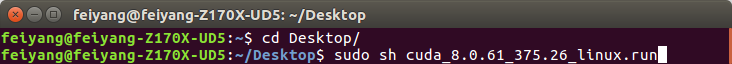
\includegraphics[scale=0.5]{./StartCUDA.png}
		\caption{\label{Fig:StartCUDA}Start CUDA installation}
	\end{figure}
	
	Then, it will go to "End User License Agreement", and you can press "CTRL + C" skip this part. And then, you need to choose some options about installation, which is shown as Fig.\ref{Fig:QuestionsCUDA}. 
	
	\begin{figure}[http]
		\centering
	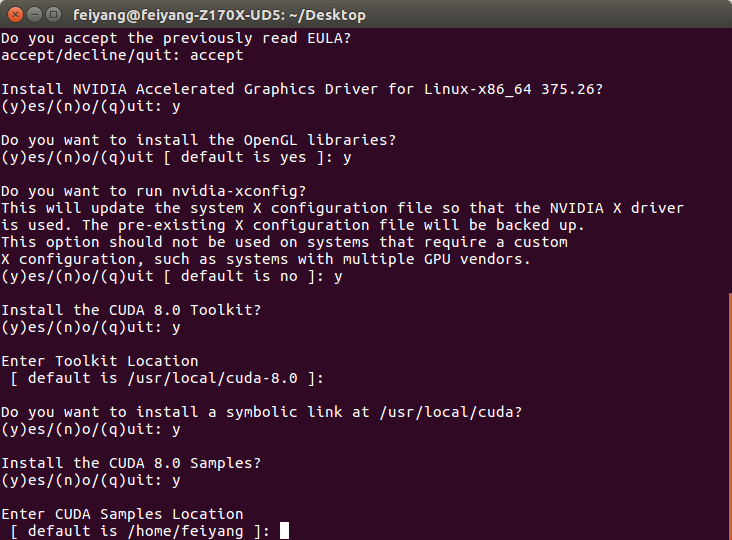
\includegraphics[scale=0.5]{./QuestionsCUDA.png}
		\caption{\label{Fig:QuestionsCUDA}CUDA installation options}
	\end{figure}
	
	Waiting some time till it finishes, and rebooting your system, the CUDA has already been installed. 
	
	\subsubsection{Installing cuDNN}
	Then, we can install cuDNN. Go to the \href{https://developer.nvidia.com/cudnn}{cuDNN download page},and download the cuDNN file you need, as the Fig.\ref{Fig:cuDNNPage} shown. Here, we download the cuDNN v6.0 for CUDA 8.0 and Linux.
	
 

	When it finishes, uncompress cuDNN and copy the files to the directory of CUDA you installed before by command below,
	
	\begin{lstlisting}{frame=single, language=bash}
	$ cd Desktop/
	$ tar xvzf cudnn-8.0-linux-x64-v6.0.tgz
	$ sudo cp cuda/include/cudnn.h /usr/local/cuda/include
	$ sudo cp cuda/lib64/libcudnn* /usr/local/cuda/lib64
	$ sudo chmod a+r /usr/local/cuda/include/cudnn.h \
		/usr/local/cuda/lib64/libcudnn*
	\end{lstlisting}
	
	Till now, we finish installing the cuDNN. Now we can start to install TensorFlow.
	
		\begin{figure}[http]
		\centering
		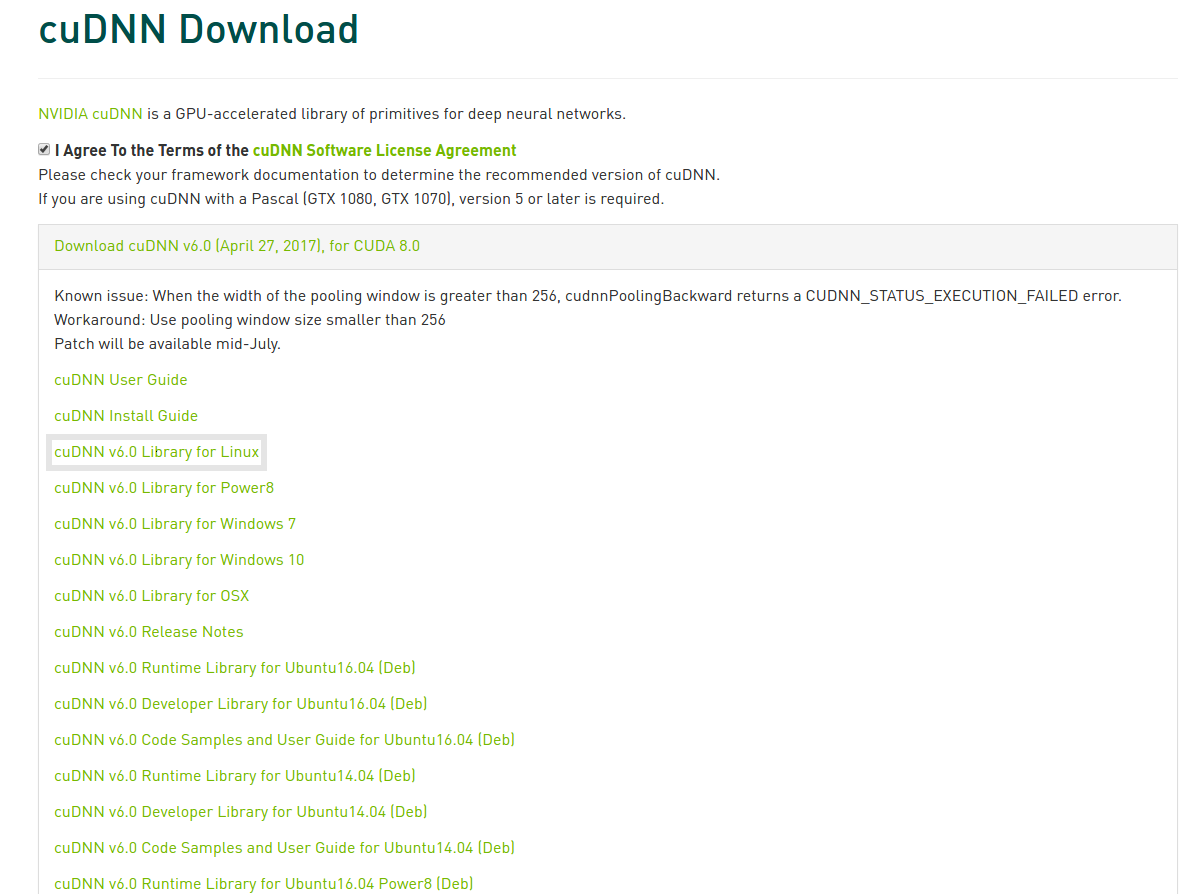
\includegraphics[scale=0.35]{./cuDNNPage.png}
		\caption{\label{Fig:cuDNNPage}cuDNN download page}
	\end{figure} 
	\subsection{Installing TensorFlow}
	\label{sec:InstallationTensorFlow}
	On the \href{https://www.tensorflow.org/install/install_linux}{TensorFlow official installation tutorial}, it introduces 4 ways to install TensorFlow. Here, we suggest you use the Anaconda, which will make the programing easier. For other ways, please refer \href{https://www.tensorflow.org/install/install_linux}{TensorFlow official installation tutorial}.
	\subsubsection{Installing Anaconda}
	At first, we need to install the Anaconda. Go to the \href{https://www.continuum.io/downloads}{Anaconda download page}, and you need to choose which version of Python you will use. Here, we choose \href{https://repo.continuum.io/archive/Anaconda3-4.4.0-Linux-x86_64.sh}{64-BIT(X86) INSTALLER}. \par
	Then, install Anaconda with the command below.\par
	For Python 3.6 version,
	\begin{lstlisting}{frame=single, language=bash}
	$ cd Desktop/
	$ bash Anaconda3-4.4.0-Linux-x86_64.sh
	\end{lstlisting}
	For Python 2.7 version,
	\begin{lstlisting}{frame=single, language=bash}
	$ cd Desktop/
	$ bash Anaconda2-4.4.0-Linux-x86_64.sh
	\end{lstlisting}
	It is easily to install	it, we don't want to talk it any more.
	
	\subsubsection{Installing TensorFlow with Anaconda}
	Now we can start install TensorFlow eventually with Anaconda. \par
	First, open the terminal and create a conda environment named \textbf{tensorflow} by invoking the following command:
	\begin{lstlisting}{frame=single, language=bash}
	$ conda create -n tensorflow
	\end{lstlisting}	
	
	Then activate the conda environment created above by:
	\begin{lstlisting}{frame=single, language=bash}
	$ source activate tensorflow
	\end{lstlisting}
	
	At last, install the TensorFlow inside your conda environment:
	\begin{lstlisting}{frame=single, language=bash}
	$ pip install --ignore-installed --upgrade TF_PYTHON_URL
	\end{lstlisting}
	
	where \textbf{TF\_PYTHON\_URL} is the \href{https://www.tensorflow.org/install/install_linux#the_url_of_the_tensorflow_python_package}{URL of the TensorFlow Python package}. You should take care the Python version and the CPU or GPU version. For example, the following command installs the GPU version of TensorFlow for Python 3.6:
	
	\begin{lstlisting}{frame=single, language=bash}
	$ pip install --ignore-installed --upgrade \
		https://storage.googleapis.com/tensorflow/linux/gpu\
		/tensorflow_gpu-1.1.0-cp36-cp36m-linux_x86_64.whl
	\end{lstlisting}
	
	\subsection{Validating your installation}
	At last, we need to run a short TensorFlow program to validate your installation. \par
	Invoke Python from your shell as follows:
	\begin{lstlisting}{frame=single, language=bash}
	$ python
	\end{lstlisting}
	
	Enter the following short program inside the Python interactive shell: \par
	\begin{python}
		>>> import tensorflow as tf
		>>> hello = tf.constant('Hello, TensorFlow!')
		>>> sess = tf.Session()
		>>> print(sess.run(hello))
		\end{python}
	
	If the systems outputs the following, then you are ready to begin writting TensorFlow programs:
	\begin{python}
		Hello, TensorFlow!
		\end{python}
	\section{Linear Regression}
		\label{sec:LinearReg}
	
		Now, we can start our first TensorFlow program: Linear Regression. I believe this is a good start for your TensorFlow study. \par
		There are two parts in this section. First, we need to install an IDE for programming. Here, the PyCharm is introduced as a powerful IDE for Python, and we will explain how to install and deploy it. Of course, you can choose other IDEs, and you can skip to the \hyperref[sec:LinearRegProgram]{Linear Regression Program}.
		
	\subsection{Installing PyCharm}
	
	\href{https://www.jetbrains.com/pycharm/}{Pycharm} is a powerful IDE for Python programming, but it is a little heavy. You can download the \href{https://www.jetbrains.com/pycharm/download/download-thanks.html?platform=linux&code=PCC}{community version} or apply student-free \href{https://www.jetbrains.com/pycharm/download/download-thanks.html?platform=linux}{professional version}. \par
	When you finishing it, you can install the Pycharm by invoking the following command:
	\begin{lstlisting}{frame=single, language=bash}
	$ cd Desktop/
	$ tar -xzf pycharm-professional-2017.1.4.tar.gz
	$ mv pycharm-2017.1.4/ ~/
	$ cd ~/pycharm-2017.1.4/bin/
	$ sh pycharm.sh
	\end{lstlisting}
	
	Now, open the Pycharm and configure the setting. Click "File" and "Default Settings" . Then click "Project Interpreter", choose the Python interpreter in "tensorflow" environment, as the Fig.\ref{Fig:PycharmSetting} shown.
	
	\begin{figure}[http]
		\centering
		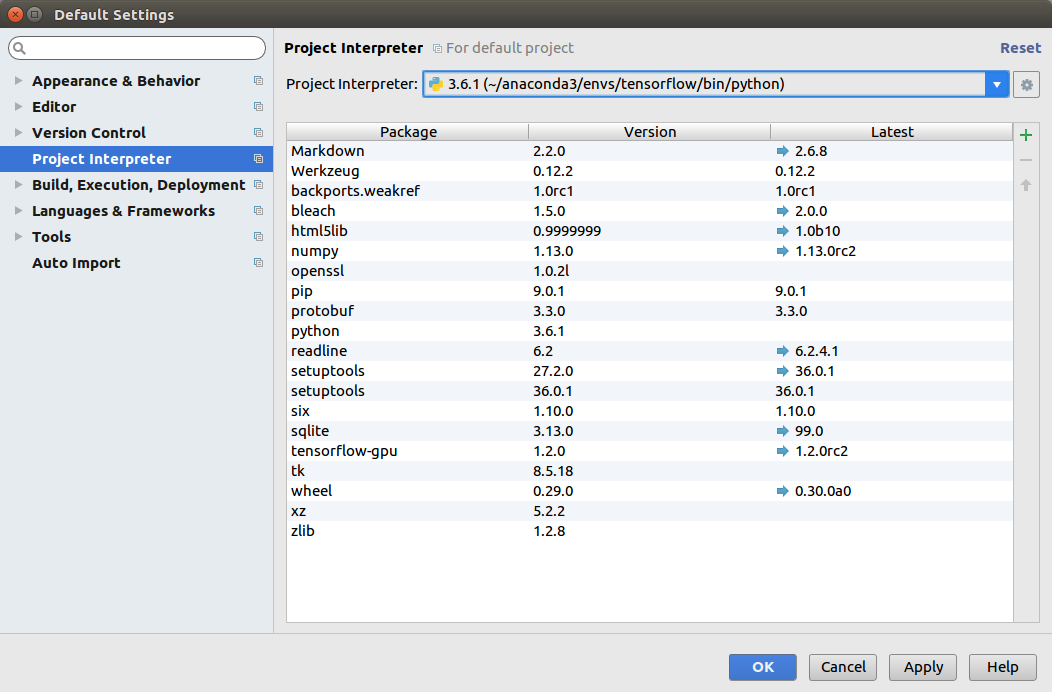
\includegraphics[scale=0.35]{./PycharmSetting.png}
		\caption{\label{Fig:PycharmSetting}Pycharm interpreter settings}
	\end{figure}
		Now, the settings for Pycharm are all done. 
	\subsection{Linear Regression Program}\
	\label{sec:LinearRegProgram} 
	
	Now we can start our first TensorFlow program, Linear Regression. Our task is find a best line to fit all the points in the X-Y plane. \par
	At first, we need to import the "tensorflow" module to the Python, and also "numpy" for scientific computing, "matplotlib" for 2D figure plotting. The code is shown below:
	\begin{python}
		import tensorflow as tf
		import numpy as np
		import matplotlib.pyplot as plt  
	\end{python}
		
	Then generating a sets of data as the training set by "numpy", which is 2 dimensions. "x\_data" is 100 evenly spaced numbers between 0 to 1. "y\_data" has the linear relationship with "x\_data". In order to make it a little hard to learn, we add some noise to the "y\_data". The code is shown below:
	\begin{python}
		x_data = np.float32(np.linspace(0, 1, 100)) 
		x_data = x_data.reshape(1, 100)
		y_data = 0.5 * x_data + 0.2 + np.random.normal(0, 0.01, 100)
	\end{python}

	Then we need to create a linear model using the TensorFlow, "W" and "b" stand for the wight  and the bias of the linear equation. The initial value of bias is 0 and the weight is a random variable from uniform distribution. "y" is the out in our model. The code is shown below:
	 \begin{python}
		b = tf.Variable(tf.zeros([1]))
		W = tf.Variable(tf.random_uniform([1,1], -1.0, 1.0))
		y = tf.matmul(W, x_data) + b
	 \end{python}
 
 	In our task, we need to train the model we created here to fit the training set. In other words, we need to make the difference between "y\_data" {\textemdash} the training target  and "y" {\textemdash} the model output small. Here, the "loss" is the variance to measure the difference. \par
 	The gradient descent algorithm is used as the optimizer, and the learning rate is 0.5. The code is shown as below.
 	\begin{python}
 		loss = tf.reduce_mean(tf.square(y - y_data))
 		optimizer = tf.train.GradientDescentOptimizer(0.5)
 		train = optimizer.minimize(loss)
 	\end{python}
 
 	Now, we can start train our training. At first, we need to initial our variables in model, and iterate the model 201 times. Every 20 iterations the program will print the model parameters. The code is shown below: \newpage
 	\begin{python}
 	init = tf.global_variables_initializer()
 	sess = tf.Session()
 	sess.run(init)
 	
 	for step in range(0, 201):
 			sess.run(train)
 			if step % 20 == 0:
 					print(step, sess.run(W), sess.run(b))
 	\end{python}
 	
	Actually, we have already get the training result from the last iteration. In order to see the it more intuitively, let's draw the result in the figure, which is shown in Fig.\ref{Fig:FigResult}. Also, the code is attached below:
	
	\begin{python}
		y_estimated = sess.run(W) * x_data + sess.run(b)
		x_data = x_data.reshape(100)
		y_data = y_data.reshape(100)
		y_estimated = y_estimated.reshape(100)
		plt.axis([0,1,0,0.8])
		plt.plot(x_data,y_data,'b.')
		plt.plot(x_data, y_estimated,'r-')
		plt.show()
	\end{python} 
		\begin{figure}[http]
		\centering
		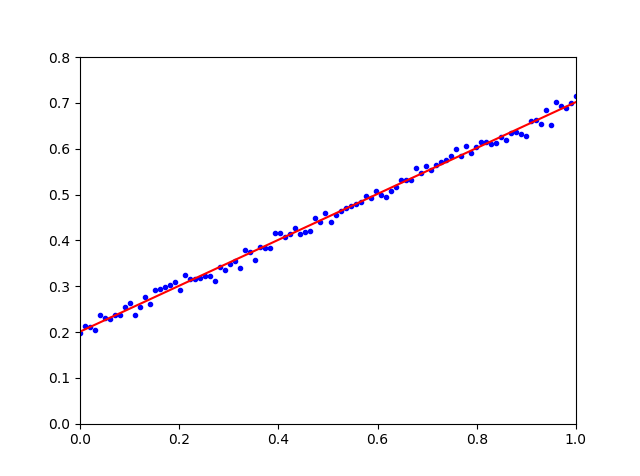
\includegraphics[scale=0.65]{./FigResult.png}
		\caption{\label{Fig:FigResult}Linear Regression Result}
	\end{figure}

	Till now, we finish the our first TensorFlow program {\textemdash} Linear Regression.
\end{document}